\clearpage
%\setcounter{page}{1}
\maketitlesupplementary

\section{Gaussianity preservation of our noise warping algorithm}

In this section, we discuss our noise warping algorithm, providing a formal proof of its Gaussianity preservation properties. We also present an illustrative example that demonstrates how noise that undergoes expansion and subsequent contraction returns to its original state, showcasing how our noise warping algorithm maintains the underlying Gaussian distribution throughout the warping process.

\begin{proof}
    For each $(x,y) \in V$, $R(x,y)$ is a collection of upsampled noise $X_i$, where
    \begin{align*}
    \bE[X_i] &= \bE[\frac{q(x,y)}{d}] + \bE[\frac{1}{\sqrt{d}}(Z_i - \frac{S}{d})] = 0  \\
        \Var(X_i) &= \Var(\frac{q(x,y)}{d}) + \Var(\frac{1}{\sqrt{d}}(Z_i - \frac{S}{d})) \\
        &= \frac{1}{d^2} + \frac{1}{d} \Var(\frac{d-1}{d}Z_i - \sum_{j\neq i} \frac{Z_j}{d}) \\
        &= \frac{1}{d^2} + \frac{1}{d} \frac{(d-1)^2 + (d-1)}{d^2} = \frac{1}{d},
    \end{align*}
    where we used the fact that $q(x,y)$ and $Z_i$'s are i.i.d. standard Gaussians.
    Since $X_i$ is constructed as a weighted sum of Gaussians, itself is also a Gaussian.
    Moreover, for $i \neq j$, we compute
    \begin{align*}
        &\Cov(X_i, X_j) \\
        =&\Cov(\frac{q(x,y)}{d} + \frac{1}{\sqrt{d}}(Z_i - \frac{S}{d}), \frac{q(x,y)}{d} + \frac{1}{\sqrt{d}}(Z_j - \frac{S}{d})) \\
        =& \frac{1}{d^2} + \frac{1}{d}\bE[(Z_i - \frac{S}{d})(Z_j - \frac{S}{d})] \\
        =& \frac{1}{d^2} + \frac{1}{d}(0 - 2 \frac{\bE[Z_i S]}{d} + \frac{\bE[S^2]}{d^2}) \\
        =& \frac{1}{d^2} + \frac{1}{d}(-\frac{2}{d} + \frac{1}{d}) = 0.
    \end{align*}
    Hence all $X_i$'s are independent.

    For each $(x',y') \in V'$, if $\deg_G((x',y')) = 0$, then $q'(x',y')$ is sampled as an independent standard Gaussian. 
    Otherwise, the output noise pixel $q'(x',y')$ is built as a weighted sum of $R(x,y)\text{.pop}()$ for each edge $((x,y), (x',y'))\in E$, where $R(x,y)\text{.pop}()$ is an independent Gaussian of mean 0 and variance $\frac{1}{\deg_G((x,y))}$.
    Hence $q'(x',y')$ is also a Gaussian with mean 0.
    The variable $s$ after executing the inner for loop thus represents the variance of $q'(x',y')$, so the renormalization at the end brings $q'(x',y')$ back to a standard Gaussian.
    Since the composing $X_i$'s are independent, the resulting noise $q'$ should also have an independent Gaussian in each pixel.
\end{proof}

\begin{example}[Exact recovery of \expansion-\contraction]
Consider the following evolution of noise across three frames with forward flows $f_{i\to j}$ going from frame $i$ to frame $j$ with $i + 1 = j$ (and backward flow if $i -1 = j$).
Suppose at frame $1$, a pixel $v \in D$ with density $1$ has noise $q$. Suppose further that $v'_a$ is a pixel at frame $2$ such that $f_{1\to 2}^{-1}(v'_a) = \{v\}$, and $v'_b \in D$ is the only pixel at frame $2$ such that $f_{1\to 2}^{-1}(v_b') = \varnothing$ and $f_{2\to 1}(v'_b) = v$.
This represents the scenario where $v$ is expanded into two pixels $v'_a,v'_b$.
Then \cref{alg:main} with forward flow $f_{1\to 2}$ and backward flow $f_{2 \to 1}$ will result in $v'_a$ having density $1/2$ and noise $\frac{q}{2} + \frac{1}{\sqrt{2}}(\frac{Z_a-Z_b}{2})$, and $v_b'$ having density $1/2$ and noise $\frac{q}{2} + \frac{1}{\sqrt{2}}(\frac{Z_b-Z_a}{2})$, where $Z_a$ and $Z_b$ are i.i.d. standard Gaussians.
Now, from frame $2$ to frame $3$, suppose there exists a pixel $v''$ such that $f_{2\to 3}^{-1}(v'') = \{v'_a,v'_b\}$, i.e., they both $v'_a$ and $v'_b$ contract to $v''$, and that $f_{3\to2}(D) \cap \{v'_a,v'_b\} = \varnothing$.
Then \cref{alg:main} with forward flow $f_{2\to 3}$ and backward flow $f_{3\to 2}$ will result in $v''$ having density $1$ and noise $q$, hence deterministically recovering the noise and density of $v$ in frame 0.

\end{example}


\section{Qualitative results of training-free image diffusion based video editing}

Noise warping methods that do not preserve Gaussianity degrade per-frame performance, as originally pointed out in~\cite{chang2024warped}. For example, using nearest neighbor and bilinear interpolation destroys the Gaussianity (see \cref{fig:supp_warped_noise_flow_vis}) and consequently deteriorates the per-frame performance on pre-trained image-to-image diffusion models (see \cref{fig:supp_davis_deepfloyd} and \cref{fig:supp_diffrelight_noisewarp}).

\begin{figure*}
    \centering
    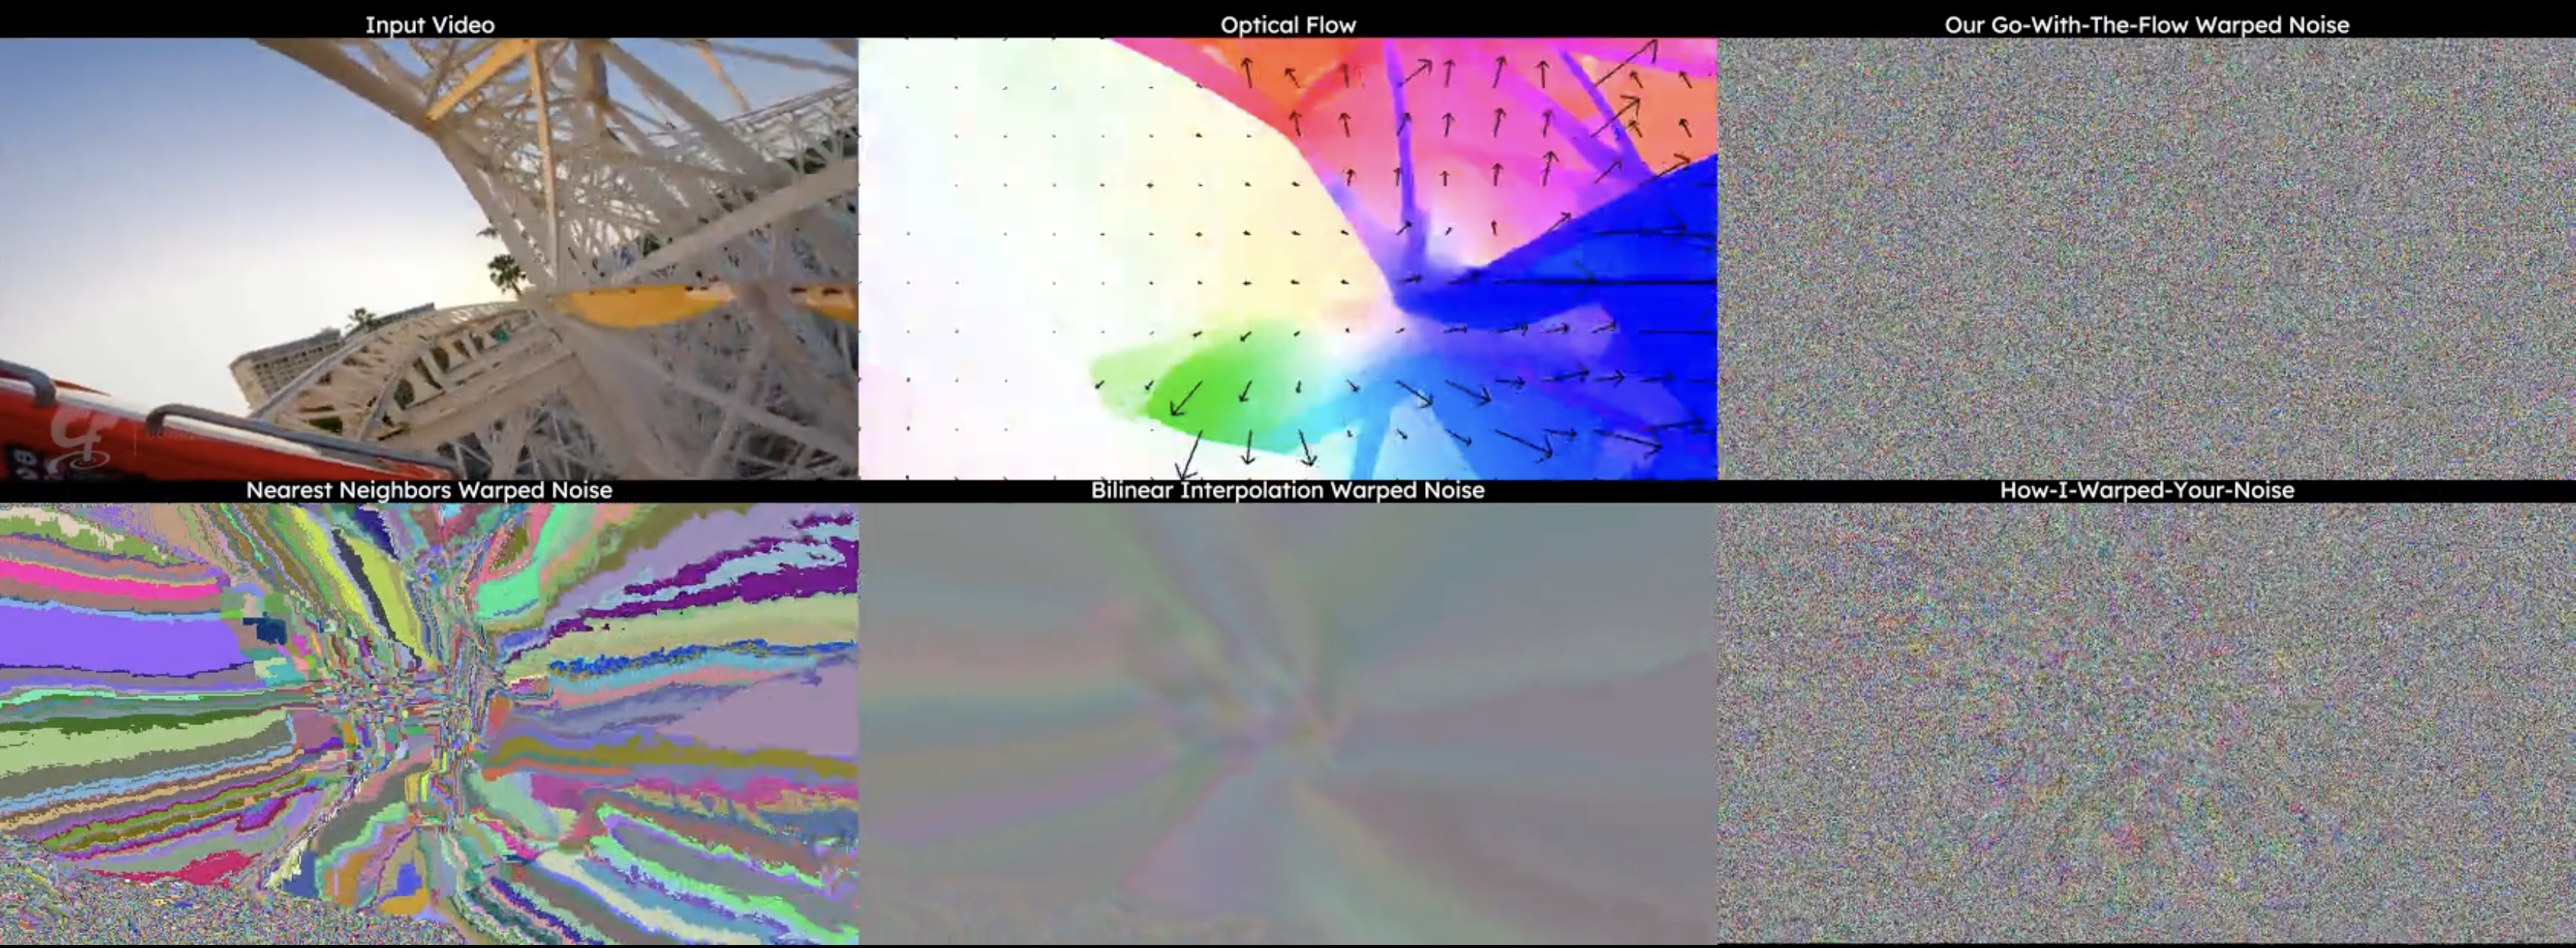
\includegraphics[width=1\linewidth]{fig/nongauss_vis.png}
    \caption{A direct visualization of the noise produced by our noise warping algorithm, HIWYN~\cite{chang2024warped}, bilinear, and nearest neighbor interpolations. The forward movement in this long roller-coaster video forces the noise to expand significantly. Early in the video, the HIWYN baseline produces visibly non-Gaussian results. See the full video on our \href{https://eyeline-research.github.io/Go-with-the-Flow/}{webpage}.}
    \label{fig:supp_warped_noise_flow_vis}
\end{figure*}

\begin{figure}
    \centering
    \includegraphics[width=1\linewidth]{fig/stroller_frame20.png}
    \caption{Using different noise warping algorithms on DeepFloyd~IF for video super-resolution on the DAVIS dataset.}
    \label{fig:supp_davis_deepfloyd}
\end{figure}

\begin{figure}
    \centering
    \includegraphics[width=1\linewidth]{fig/naz_diffrelight_grid11.jpg}
    \caption{Using different noise warping algorithms on DifFRelight for portrait video relighting. }
    \label{fig:supp_diffrelight_noisewarp}
\end{figure}


\section{The advantage of noise warping}

By using noise warping as a condition for motion, we effectively discard all structural information from our input video that cannot be inferred from motion alone. This can be advantageous, as demonstrated in \cref{fig:supp_windmill}. MotionClone does not use optical flow to guide the video trajectory, instead relying on manipulating activations within the diffusion model. As a result, the windmill gains an extra set of arms, whereas our method, which relies solely on motion information from optical flow via warped noise, does not introduce such artifacts.

\section{Comparison to the video diffusion base model without finetuning}

Interestingly, video diffusion models respond to noise warping even without training. In \cref{fig:supp_windmill} the rightmost column, even though the per-frame quality suffers, the flow of the output video still roughly follows the flow of the warped noise. However, because warped noise is statisically distinct from the pure Gaussian noise CogVideoX was trained on, without fine-tuning it can result in visual artifacts.

\section{User study settings and statistics}
\label{sec:supp_user_study}

\cref{fig:supp_user_study_screenshots_statistics} presents our user study questionnaires and statistics for two applications: (1) local object motion control, and (2) turnable camera movement video generation. Our questions focus on users' overall subjective preference, controllability, and temporal consistency.

\section{Model Agnostic}


Our method is data- and model-agnostic. It can be used to add motion control to arbitrary video diffusion models by only processing the noise sampling during fine-tuning. For example, it also works with AnimateDiff \cite{guo2024animatediff} fine-tuned on the WebVid dataset~\cite{Bain21} (the weights for this model on our \href{https://github.com/Eyeline-Research/Go-with-the-Flow}{GitHub} page). See its qualitative results in \cref{fig:supp_animatediff_grid}. Since release, the community has also trained a version of Go-with-the-Flow on HunyuanVideo (linked on our \href{https://github.com/Eyeline-Research/Go-with-the-Flow}{GitHub} page). Therefore, our method will generalize to future more advanced video diffusion base model.

\section{Pseudo code}

See \cref{listing:supp_algo_pseudo_code} for our noise warping pseudo code. See our source code and model checkpoints on \href{https://github.com/GoWithTheFlowPaper/gowiththeflowpaper.github.io}{GitHub}.

\begin{figure*}
    \centering
    \includegraphics[width=0.7\linewidth]{fig/windmills.pdf} 
    \caption{
    We show a \cutndrag~animation of a windmill rotating clockwise, next to the derived optical flow, our outputs, a baseline and an ablation. \textbf{Note} that the input video column appears to have two sets of panels because it's being cut and dragged over itself to create rotational motion. \textbf{When using noise warping is better}: Per-frame structural information can poison the result of MotionClone, giving the windmill an extra set of arms - whereas ours only receives motion information from optical flow alone via warped noise (there are no double-windmills in the optical flow patterns). \textbf{Ablation in rightmost column}: warped noise with $\deglevel=.5$ on the CogVideoX base model before we fine-tune it. Because warped noise is statisically distinct from the pure Gaussian noise CogVideoX was trained on, without fine-tuning it can result in visual artifacts. Note how although the per-frame quality suffers here, it still picks up on motion queues from the warped noise (the camera zooms into the windmill).}
    \label{fig:supp_windmill}
\end{figure*}

\begin{figure*}
    \centering
    \begin{subfigure}{.48\linewidth}
    \includegraphics[width=\linewidth]{fig/user_study_screenshot_1.png}
    \subcaption{User study interface and questions for local object motion control, corresponding to ~\cref{fig:comparisons_video_diffusion_object_motions} in the main paper.}
    \end{subfigure}
    \hfill
    \begin{subfigure}{.48\linewidth}
    \includegraphics[width=\linewidth]{fig/user_study_screenshot_2.png}
    \subcaption{User study interface and questions for turnable camera movement video generation, corresponding to ~\cref{fig:comparisons_video_diffusion_turning_object} in the main paper.}
    \end{subfigure}
    \\[12pt]
    \begin{subfigure}{0.48\linewidth}
    \centering
    \includegraphics[width=.7\linewidth]{fig/user_study_1_statistics_1.png}
    \subcaption{User study statistics for local object motion control on the first question ``\textit{Which video is the best overall?}''}
    \end{subfigure}
    \hfill
    \begin{subfigure}{0.48\linewidth}
    \centering
    \includegraphics[width=.7\linewidth]{fig/user_study_1_statistics_2.png}
    \subcaption{User study statistics for local object motion control on the second question ``\textit{Which video best aligns with the user intent for controlling the object movement based on the input?}''}
    \end{subfigure}
    \\[12pt]
    \begin{subfigure}{0.48\linewidth}
    \centering
    \includegraphics[width=.7\linewidth]{fig/user_study_1_statistics_1.png}
    \subcaption{User study statistics for local object motion control on the third question ``\textit{Which video best preserves the intended camera movement from the input?}''}
    \end{subfigure}
    \hfill
    \begin{subfigure}{0.48\linewidth}
    \centering
    \includegraphics[width=.7\linewidth]{fig/user_study_1_statistics_1.png}
    \subcaption{User study statistics for local object motion control on the fourth question ``\textit{Which video maintains the most consistent and stable motion throughout?}''}
    \end{subfigure}
    \\[12pt]
    \begin{subfigure}{0.48\linewidth}
    \centering
    \includegraphics[width=0.7\linewidth]{fig/user_study_2_statistics_1.png}
    \subcaption{User study statistics for motion transfer on the first question ``\textit{Which video has better overall quality?}''}
    \end{subfigure}
    \caption{User study questionnaires screenshots and statistics. For all the questions of both applications, our method (the rightmost bar plot) significantly wins the most user preferences.}
    \label{fig:supp_user_study_screenshots_statistics}
\end{figure*}

% \begin{figure*}
%     \centering
%     \includegraphics[width=1\linewidth]{fig/animatediff.jpg}
%     \caption{Fine-tuning AnimateDiff with our warped noise flow. All rows share the same movements, and all columns share the same text prompts. The first column is the reference video providing the flow to warp the noise in column 2, which is then used to diffuse all videos to the right. Please zoom in to see the captions for each row (input videos driving movement and warping noise via optical flow) and each column (text prompt for each video cell). Refer to our project video to see these in animation form.}
%     \label{fig:supp_animatediff_grid}
% \end{figure*}

\begin{figure*}
    \centering
    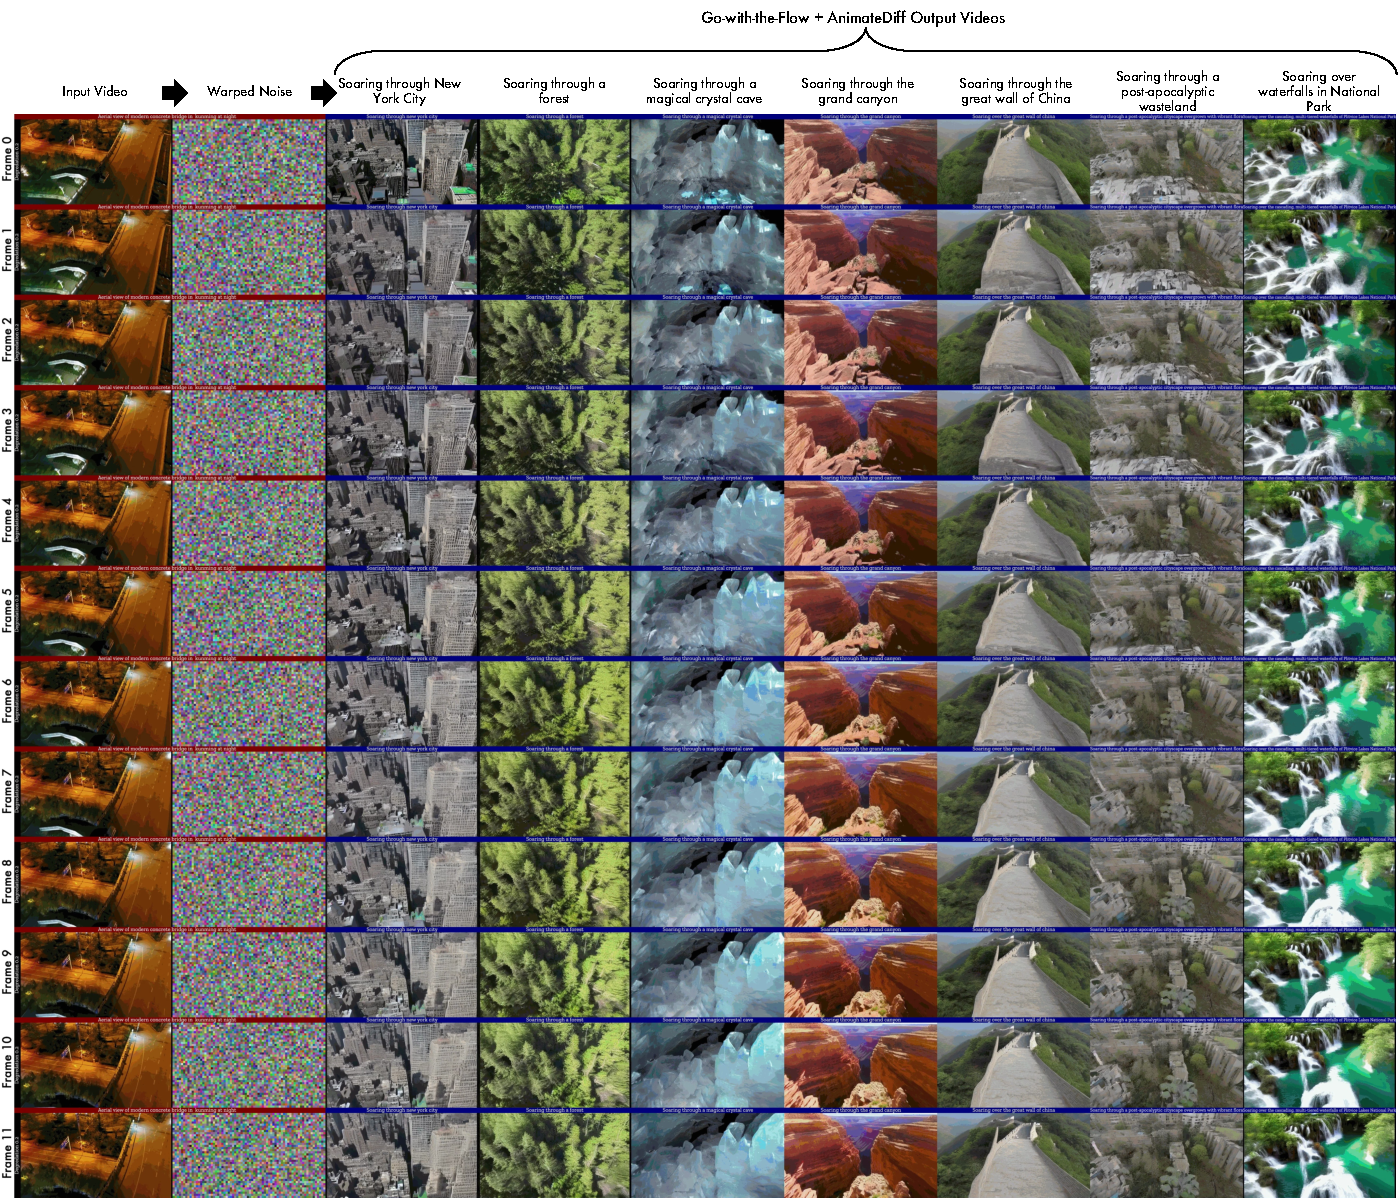
\includegraphics[width=1\linewidth]{fig/AnimateDiffAnimation.pdf}
    \caption{Fine-tuning AnimateDiff with our warped noise flow. We used Go-with-the-Flow to fine-tune AnimateDiff T2V, and display the results above. The input video is on the left, and from that video we derive warped noise which is used to initialize AnimateDiff on the columns to its right with different text prompts.}
    \label{fig:supp_animatediff_grid}
\end{figure*}

\begin{figure*}
\begin{lstlisting}
def warp_noise(prev_frame, cur_frame, prev_noise, prev_weight):

    height, width, _ = prev_frame.shape

    flow = optical_flow(prev_frame, cur_frame) # Agnostic to the optical flow algorithm
    backwards_flow = -flow # A cheap approximation of optical_flow(cur_frame, prev_frame)

    expansion_noise    = zeros(height, width)
    contraction_noise  = prev_noise.copy()

    expansion_mask     = ones (height, width, type=bool)
    contraction_mask   = zeros(height, width, type=bool)

    for x in range(width): for y in range(height):
        dx, dy = flow[x,y]
        if 0 <= x+dx <= width-1 and 0 <= y+dy <= height-1:
            # This particle stays in bounds
            expansion_mask  [x+dx, y+dx] = False
            contraction_mask[x   , y   ] = True  # Contraction mask is True where 

    for x in range(width): for y in range(height):
        if expansion_mask[x, y]:
            dx, dy = backwards_flow[x,y]
            expansion_noise [x, y] = prev_noise[x+dx, y+dy]

    # We've decided which source pixels are involved in contraction and expansion now
    contraction_noise &= contraction_mask
    expansion_noise, contraction_noise, cur_weight = jointly_regaussianize_and_rebalance_weights(
        expansion_noise, contraction_noise, prev_weight
    ) # Regaussianize all noise values here, and divide the weights by the number of pixels in each bin

    contraction_weight = zeros(height, width)
    for x in range(width): for y in range(height):
        if contraction_mask[x, y]:
            # Contraction treats the noise pixels as particles, each moving from the source to the
            # destination with this flow
            dx, dy = flow[x,y]
            # Contraction is a weighted sum of source pixels to a destination pixel
            pixel_weight = cur_weight[x, y]
            # Sum all the source noise pixels that contract to the same destination
            contraction_noise [x+dx, y+dy] += prev_noise[x, y] * pixel_weight
            # When we multiply a noise pixel by a weight, the variance changes by that weight squared
            contraction_weight[x+dx, y+dy] += pixel_weight ** 2 
    contraction_noise /= sqrt(contraction_weight) # Adjust the variance of the summed contracted noise

    # Mixing contraction and expansion noises with their respective masks
    cur_noise = contraction_noise & contraction_mask + expansion_noise & expansion_mask

    return cur_noise, cur_weight
\end{lstlisting}
\caption{Our noise warping pseudo code.}
\label{listing:supp_algo_pseudo_code}
\end{figure*}
